\section{Tecnologie utilizzate}

Dal punto di vista delle piattaforme, degli strumenti operativi e delle pratiche di deployment, l’ambiente tecnologico osservato durante lo stage combina soluzioni \emph{enterprise} 
consolidate con strumenti e approcci moderni orientati alla scalabilità, all’integrazione e all’automazione. 
Di seguito viene fornita una descrizione estesa delle tecnologie principali e del loro impatto operativo.

\medskip
\noindent\textbf{\emph{Salesforce Commerce Cloud}}
\emph{Salesforce Commerce Cloud} insieme ai moduli \emph{Service Cloud} e \emph{Marketing Cloud} è una suite pensata per gestire vendite online, assistenza clienti e 
attività di marketing in modo integrato. Viene usata sia per soluzioni \emph{B2B} che \emph{B2C} e permette di costruire cataloghi prodotti, gestire ordini e mantenere 
aggiornati i profili dei clienti collegando la piattaforma ad altri sistemi aziendali (per esempio ERP, sistemi di magazzino o gateway di pagamento).
La piattaforma facilita la personalizzazione dell’esperienza d’acquisto grazie a regole commerciali e strumenti di segmentazione: è possibile mostrare contenuti, 
offerte e percorsi diversi a seconda del cliente o del canale. Allo stesso tempo automatizza molte attività di marketing e customer care (campagne, promozioni, 
follow-up post-acquisto e ticket di assistenza) riducendo lavoro manuale e tempi di risposta.

\begin{figure}[htbp]
    \centering
    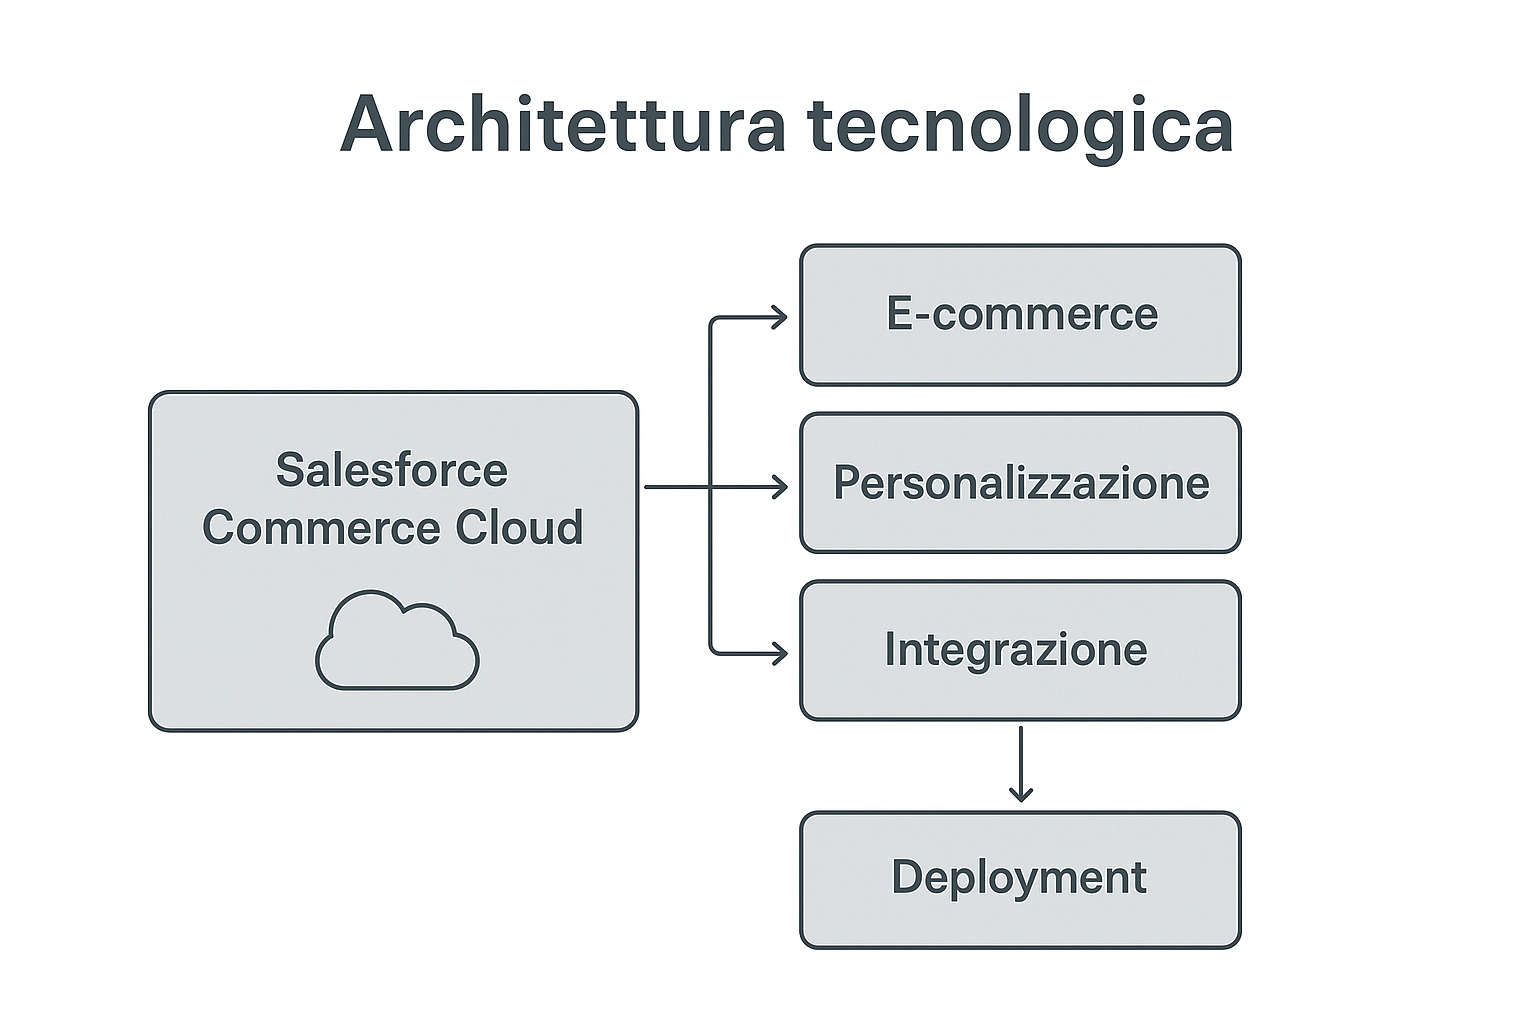
\includegraphics[width=0.8\textwidth]{azienda/architettura_tecnologica}
    \caption{Architettura tecnologica osservata: le principali piattaforme e i flussi di integrazione tra e-commerce, personalizzazione, integrazione e deployment.}
    \label{fig:architettura_tecnologica}
\end{figure}


\medskip
\noindent\textbf{\emph{Bloomreach}}
\emph{Bloomreach} è una piattaforma pensata per migliorare la ricerca interna e personalizzare la \emph{customer journey} in modo più intelligente e mirato. 
Viene impiegata soprattutto in progetti di scala per rendere le ricerche sul sito più pertinenti (per esempio mostrando risultati, suggerimenti e filtri che si adattano al contesto dell’utente) 
e per orchestrare contenuti e offerte personalizzate lungo tutto il percorso di acquisto.
Nella pratica, \emph{Bloomreach} combina segnali comportamentali, dati di prodotto e informazioni di profilo per alimentare ranking dei risultati, raccomandazioni, 
regole di \emph{merchandising} e landing page dinamiche; spesso è integrata con il \emph{CMS} (sistema per creare, gestire e pubblicare contenuti digitali senza intervento tecnico diretto) e il \emph{CRM} così da arricchire i profili utente e offrire esperienze 
realmente \emph{omnichannel} (sito, app, email e punti vendita).
I benefici tipici sono una scoperta prodotti più veloce e percorsi d’acquisto più coerenti per il cliente. Dal punto di vista operativo 
richiede però lavoro di integrazione: mappare correttamente il catalogo e i feed, definire le regole di \emph{merchandising}, impostare metriche di rilevanza e 
continuare a fare \emph{testing} per ottimizzare i risultati.

\begin{figure}[htbp]
    \centering
    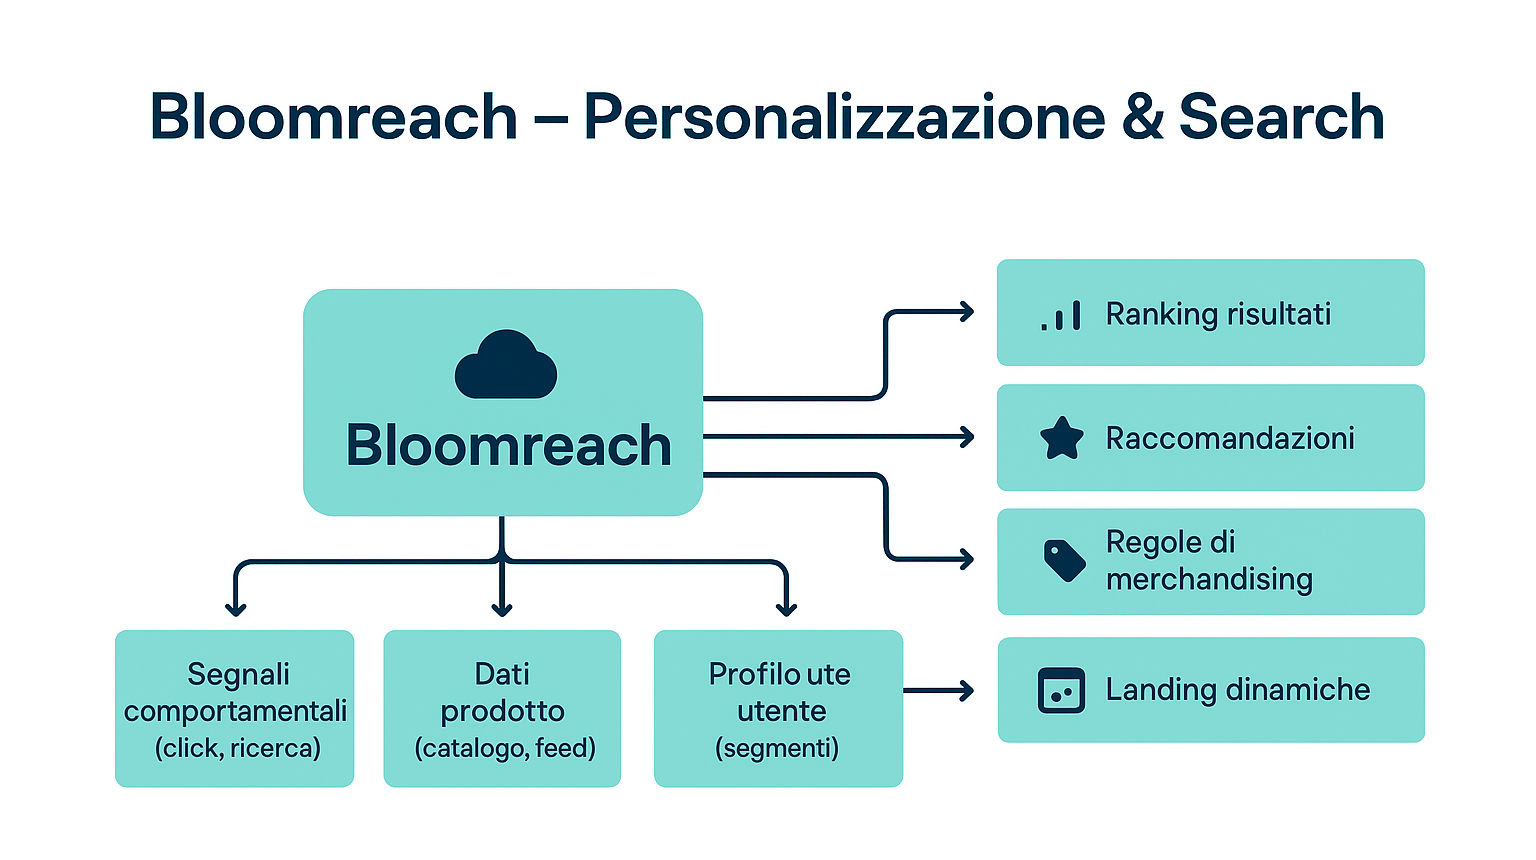
\includegraphics[width=0.8\textwidth]{azienda/bloomreach}
    \caption{Diagramma che mostra come segnali comportamentali, dati di catalogo e profili utente alimentano ranking, raccomandazioni, regole di merchandising e landing dinamiche.}
    \label{fig:bloomreach}
\end{figure}

\medskip
\noindent\textbf{\emph{deployment}}
Le piattaforme cloud e di \emph{deployment} (ad esempio \emph{AWS}, \emph{Google Cloud} e \emph{Heroku}) vengono utilizzate per ospitare le applicazioni, 
allocare risorse scalabili e creare ambienti distinti per sviluppo e collaudo (\emph{staging}) e per il traffico reale (\emph{production}). 
In pratica offrono servizi di \emph{hosting}, \emph{provisioning} delle risorse (CPU, memoria, storage) e strumenti per distribuire il codice in modo ripetibile.

Queste piattaforme sono il luogo dove risiedono i servizi applicativi, i \emph{database} e le risorse di \emph{caching}, 
e permettono di tenere separate le istanze di test da quelle in produzione per evitare impatti agli utenti. La scelta tra \emph{AWS}, \emph{Google Cloud} o \emph{Heroku} 
dipende spesso da vincoli progettuali, integrazioni richieste (per esempio con specifici servizi gestiti), competenze del team e considerazioni sui costi operativi.

Sul piano operativo si configurano meccanismi per il \emph{scaling} automatico, la distribuire del traffico, 
la gestione dei certificati \emph{TLS} per la sicurezza e sistemi di \emph{monitoring} e \emph{backup} per garantire disponibilità e resilienza. 
Inoltre si possono impostare pipeline di \emph{CI/CD} per automatizzare build, test e deployment, così da rendere le release più veloci e meno soggette a errori manuali.

Per l’infrastruttura è ormai comune l’adozione di pratiche di \emph{infrastructure as code} (strumenti che consentono il \emph{provisioning} ripetibile e tracciabile delle risorse). 

\begin{figure}[htbp]
    \centering
    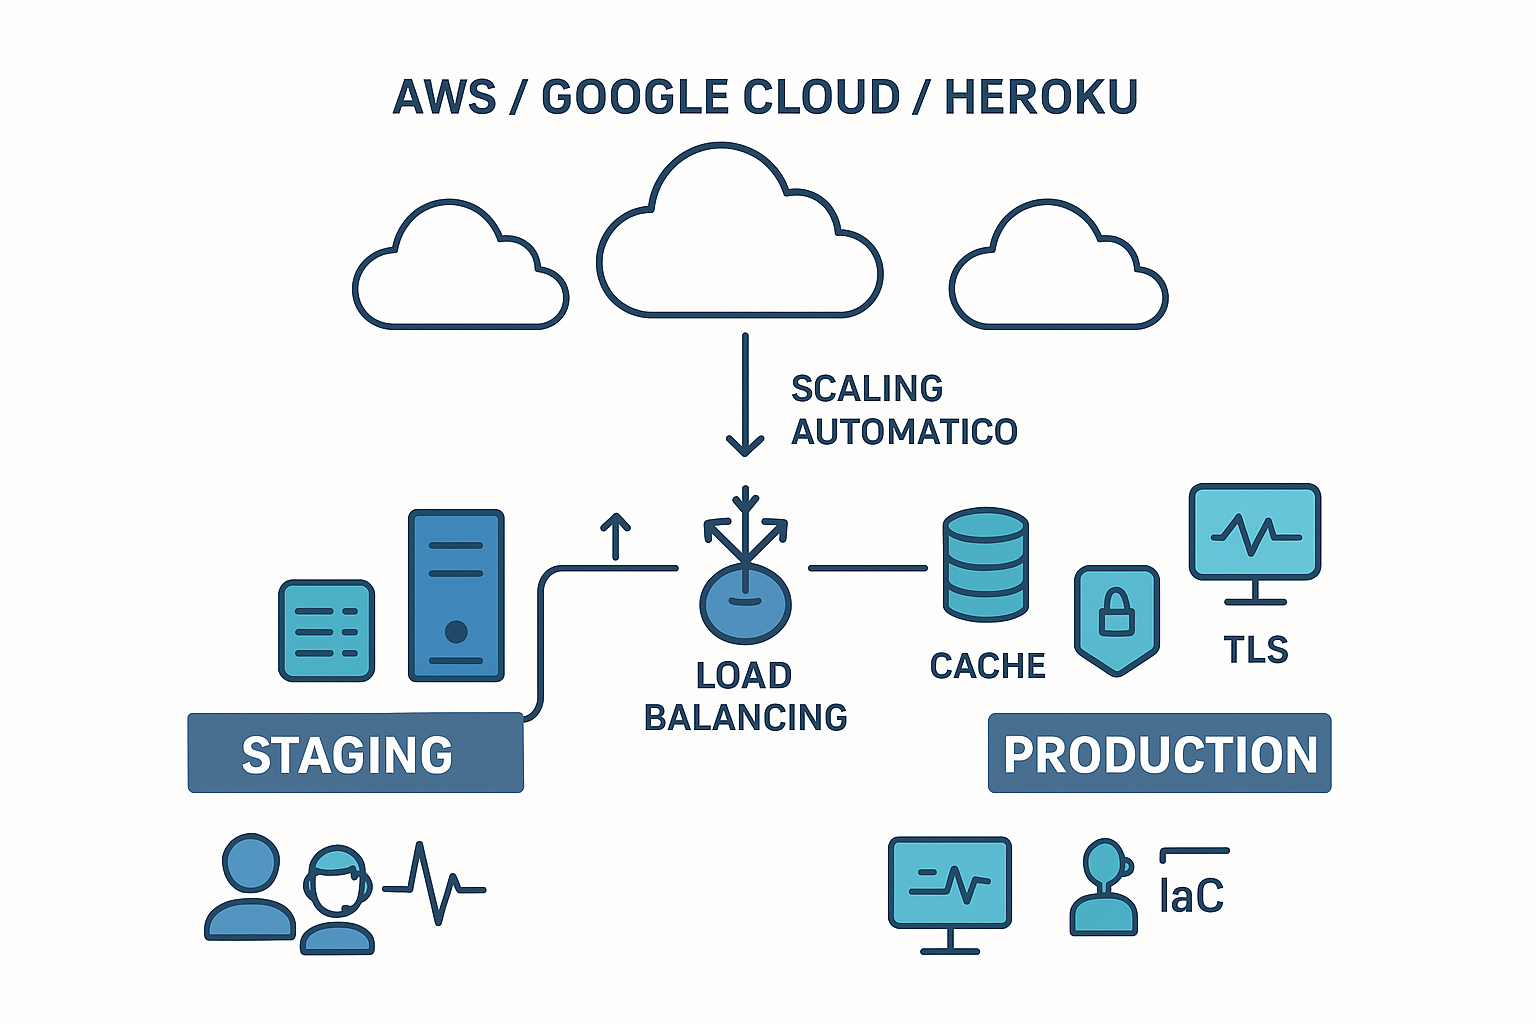
\includegraphics[width=0.8\textwidth]{azienda/deployment}
    \caption{Pipeline di integrazione e distribuzione continua: dal commit alla promozione in produzione.}
    \label{fig:deployment}
\end{figure}

% [Develop] → [Commit su Git] → [CI Build] → [Test automatici] → [Code review / Pull Request] → [Merge su main] → [Deploy su Staging] → [Verifica] → [Deploy in Production]

\medskip
\noindent\textbf{\emph{iPaaS}}
Gli strumenti di integrazione includono approcci punto a punto e soluzioni \emph{iPaaS} (\emph{Integration Platform as a Service}: piattaforme per orchestrare integrazioni) 
che collegano sistemi come \emph{CRM}, \emph{ERP}, piattaforme \emph{e-commerce} e \emph{CMS}. Mentre le integrazioni punto a punto creano connessioni dirette fra singoli sistemi, 
un \emph{iPaaS} funge da livello centrale che orchestra i flussi di dati e i processi tra più applicazioni, rendendo l'architettura più semplice da governare e manutenere.

\begin{figure}[H]
    \centering
    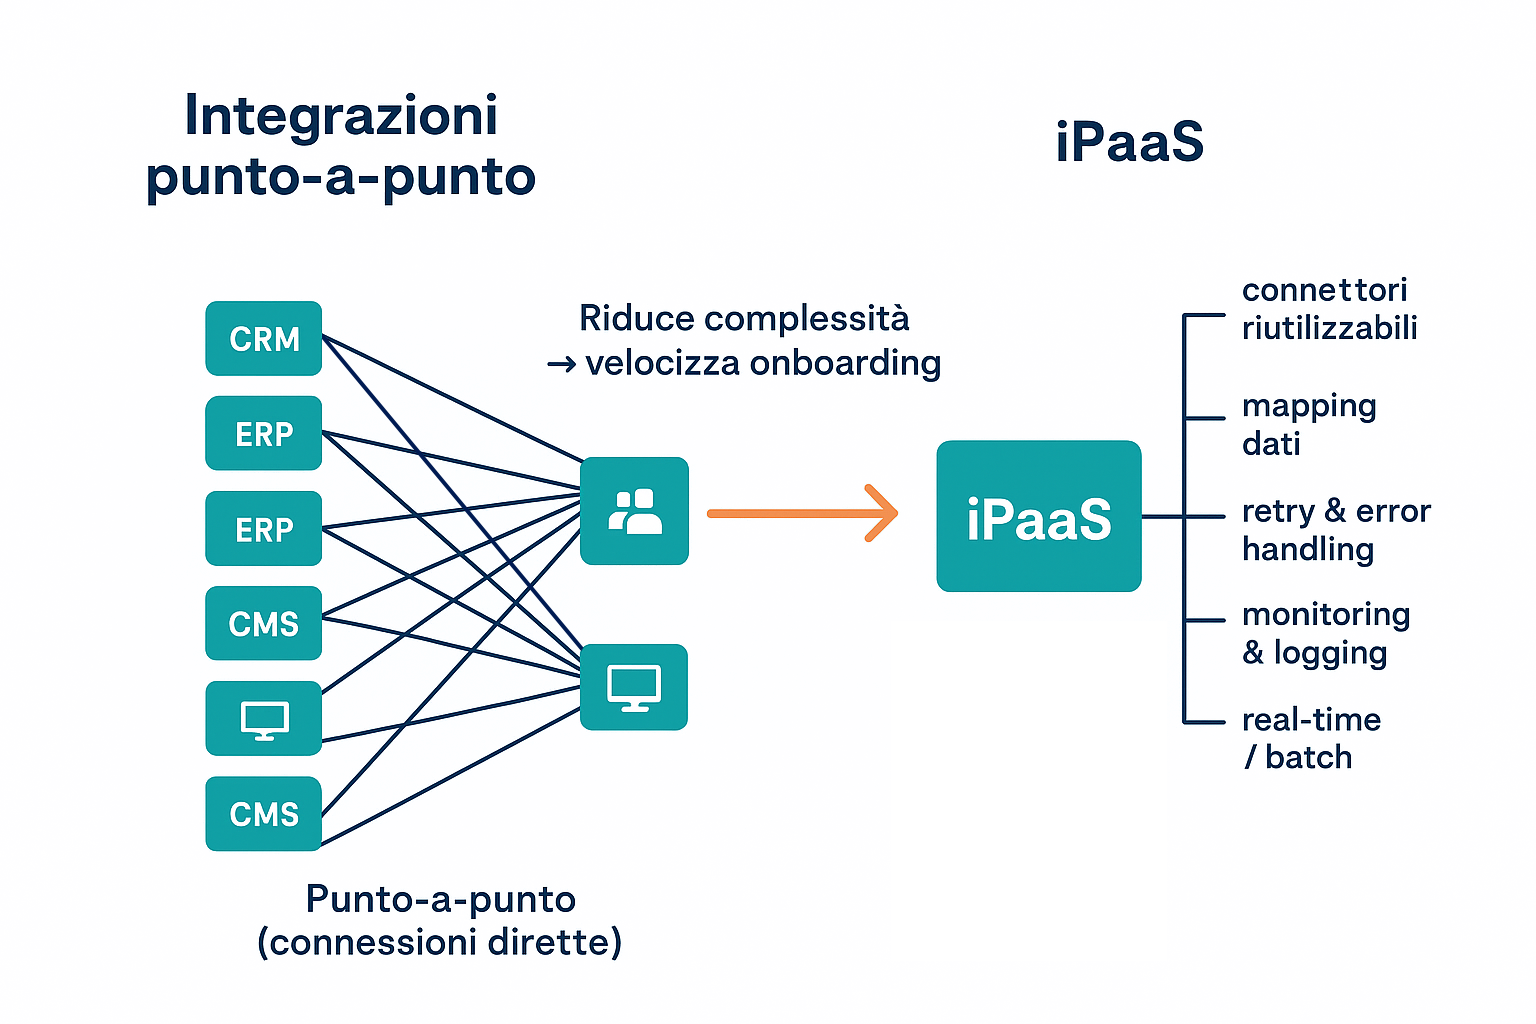
\includegraphics[width=0.8\textwidth]{azienda/iPaaS}
    \caption{Integrazioni point-to-point vs iPaaS: il diagramma mostra come un iPaaS centralizzi connettori, mapping, gestione errori e monitoring, riducendo la complessità delle integrazioni dirette e accelerando l'onboarding di nuovi sistemi.}
    \label{fig:iPaaS}
\end{figure}

L'adozione di un \emph{iPaaS} semplifica attività operative come la gestione degli \emph{endpoint} (i punti di scambio dati), la trasformazione dei \emph{payload} 
(adattamento dei formati dati), e la gestione degli errori e dei tentativi di retry (meccanismi automatici per riprovare operazioni fallite). 
Questo riduce la complessità rispetto a molte integrazioni punto a punto e velocizza l'onboarding di nuovi sistemi grazie a connettori riutilizzabili e template di integrazione.

Un \emph{iPaaS} permette anche di scegliere fra modalità di integrazione 
in tempo reale o a batch, impostare regole di mapping dei dati, e centralizzare logging e monitoraggio per individuare rapidamente problemi e colli di bottiglia.

\medskip
\noindent\textbf{Gestione progetto}
Strumenti di gestione progetto e comunicazione: \emph{Jira} per il tracciamento delle attività e \emph{Slack} per la comunicazione operativa quotidiana. \emph{Jira} 
viene usato per definire le \emph{issue} (problema, ostacolo o anomalia che richiede attenzione e risoluzione durante lo sviluppo di un progetto), assegnare priorità, documentare criteri di accettazione e tenere traccia dello stato di avanzamento; \emph{Slack} 
è lo strumento preferito per aggiornamenti rapidi e conversazioni sincrone o asincrone tra membri del \emph{team}.

\medskip
\noindent\textbf{\emph{Git}}
\emph{Git} è il fulcro del controllo versione e del coordinamento del lavoro sul codice: 
centrale non solo per conservare la storia delle modifiche, ma anche per organizzare come le nuove funzionalità arrivano nel prodotto finito. 
Nella pratica quotidiana si privilegia un flusso basato su \emph{feature branches} (ognuna per una funzionalità o correzione), 
apertura di \emph{pull request} per discutere e revisionare le modifiche (\emph{code review}) e l’uso di commit chiari e descrittivi per tracciare le decisioni.

Il processo tipico ruota attorno a poche pratiche chiave (sempre legate a \emph{Git}):
\begin{itemize}
\item sviluppo isolato su \emph{feature branches} e sincronizzazione regolare con il ramo principale per evitare divaricazioni troppo grandi;
\item revisione del codice tramite \emph{pull request} con commenti, suggerimenti e approvazioni formali prima della fusione (merge);
\item uso di convenzioni per i messaggi di commit e per i nomi dei rami (che aiutano a ricostruire la storia e a generare changelog);
\item strategie di branching consolidate (per esempio \emph{GitFlow} o approcci basati su trunk) per coordinare rilasci, hotfix e lavoro parallelo su più versioni;
\item gestione delle release tramite tag e rami dedicati alla versione (il tag identifica un punto preciso della storia come versione pubblicata);
\item pratiche di sicurezza legate a \emph{Git} (protection dei rami principali, review obbligatorie, gestione degli accessi e firma dei commit) per ridurre il rischio di errori o modifiche non autorizzate;
\item strumenti locali come le \emph{github-actions} (unità riutilizzabile di automazione che esegue compiti automaticamente in risposta a eventi del repository) e test eseguiti sul proprio ambiente prima di aprire la \emph{pull request} (ad esempio \emph{unit tests} e controlli statici), così da mantenere alta la qualità fin dal primo passo.
\end{itemize}

Dal punto di vista operativo, \emph{Git} abilita anche pratiche di rilascio sicure: le versioni vengono marcate con \emph{tag} e documentate con changelog, è possibile tornare indietro con \emph{revert} o \emph{cherry-pick} se serve correggere rapidamente una regressione, e le scelte sul tipo di merge (merge commit, fast-forward o rebase) influenzano la leggibilità della storia.

Infine, per trarre davvero vantaggio da \emph{Git} servono disciplina e coordinamento (policy per le revisioni, convenzioni condivise, role-based access) oltre a cura nella definizione dei test e nella documentazione delle release. Così, il controllo versione diventa non solo uno strumento tecnico, ma una leva organizzativa per rilasciare con più sicurezza e tracciabilità.


%\medskip

%\noindent\textbf{Implicazioni operative e suggerimenti}

%L’adozione di questo insieme di tecnologie determina alcuni vincoli e opportunità operative: la complessità delle integrazioni richiede governance dei \emph{data contracts} e 
%politiche chiare di versioning delle API; le piattaforme \emph{enterprise} come \emph{Salesforce Commerce Cloud} richiedono competenze specifiche per personalizzazioni e upgrade; 
%le risorse cloud implicano attenzione alla gestione dei costi e al monitoraggio del consumo. Per migliorare l’efficacia complessiva è raccomandabile formalizzare convenzioni comuni 
%(naming delle \emph{branches}, standard per le \emph{code review}, soglie di qualità per le \emph{pipeline}) e prevedere un minimo di documentazione operativa a supporto dell’onboarding e della manutenzione.

%In conclusione, la suite tecnologica osservata mette a disposizione strumenti potenti per costruire soluzioni integrate e scalabili; la sfida principale risiede nell’armonizzare pratiche, 
%automazioni e governance per trasformare la tecnologia in valore ripetibile e manutenibile nel tempo.


%Per la manutenzione e il supporto operativo si privilegia un approccio a livelli: monitoraggio dei servizi e dei log, 
%gestione dei \emph{ticket} tramite \emph{Jira} e interventi pianificati per aggiornamenti e patch. Nei progetti di maggiori 
%dimensioni si osserva una separazione tra team di sviluppo (feature delivery) e team di \emph{platform/operations} (monitoraggio, sicurezza, scaling), 
%mentre per clienti più piccoli le stesse persone spesso ricoprono più ruoli.

%Infine, la scelta delle tecnologie è stata chiaramente guidata dalla dimensione e dalla strategia del cliente: soluzioni \emph{Shopify} per rollout rapidi e basso \emph{TCO} 
%(\emph{Total Cost of Ownership}: costo totale di proprietà); architetture \emph{headless} e piattaforme \emph{Salesforce} per scenari enterprise e integrazioni complesse. 
%Ho inoltre riscontrato una forte propensione dell’azienda verso l’adozione di tecnologie emergenti legate all'\emph{AI} e alla personalizzazione, 
%inserite come componenti modulari (ad esempio agenti intelligenti collegati al \emph{CRM} o servizi di personalizzazione integrati con \emph{Bloomreach}). 
%In sintesi, l’ambiente tecnologico è eterogeneo e modulare, concepito per supportare sia progetti a rapido lancio sia soluzioni enterprise complesse, 
%con attenzione all’innovazione e alla scalabilità operativa.
%Sezione in cui verrà descritto il contesto produttivo in cui sono stato inserito, con particolare attenzione alle tecnologie operative viste adottare.
